La librairie Keras est une interface Python/TensorFlow\cite{tf} permetant de travailler avec des réseaux de neurones.
Ici, on ne s'attardera que sur les fonctionnalitées principales,
a savoir la création d'un réseau simple,
la regression par \sgd\ et l'évaluation des performances.


Voici un exemple de réseau de neurone assez simple
qui vas essayer de deviner l'application linéaire suivante : $f(X) = 0.2x_1 + 0.8x_2$.

\begin{figure}[H]
    \center
    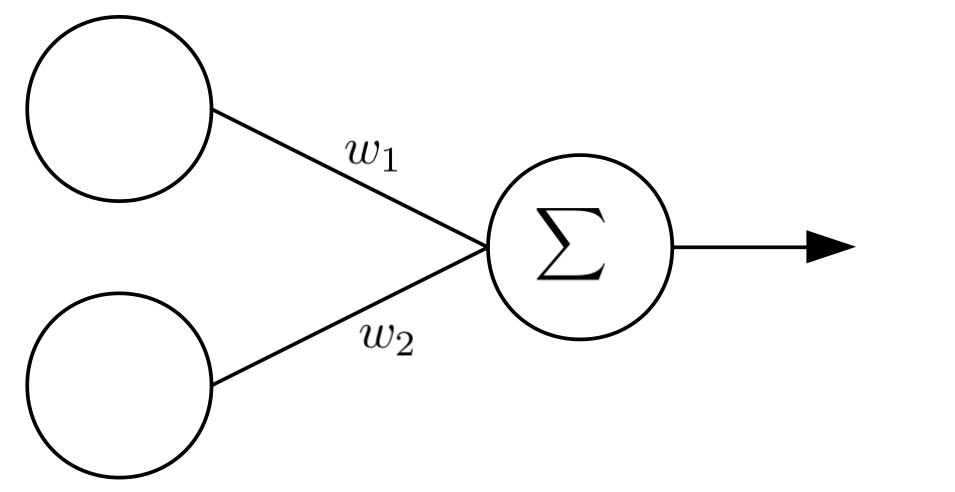
\includegraphics[height=\petit]{pict/net2.png}
	\caption{Réseau simple}
	\label{fig:net2}
\end{figure}
\vspace{-12pt}


Pour créer ce réseau et lui faire apprendre la fonction precedement citée,
le code suivant est nescessaire :
\lstinputlisting[language=Python]{code/reseau1.py}


En executant ce code, on obtient:
\begin{lstlisting}
w0 : 0.19988934695720673
w1 : 0.8001111745834351
\end{lstlisting}
On peut donc bien voir que le réseau de neurones fonctionne et
réussit à apprendre des fonctions avec plusieurs paramètres.
Il est cependant assez embetant de toujours devoir faire appel a toutes ces fonctions.
Une librairie à alors été codée afin de simplifier son utilisation.
Elle pourra être appelée avec de nombreux paramtres qui seront abordés dans les parties suivantes.\\
